\documentclass[border=2mm]{standalone}
\usepackage{tikz}
\usetikzlibrary{calc,patterns,angles,quotes}
\begin{document}
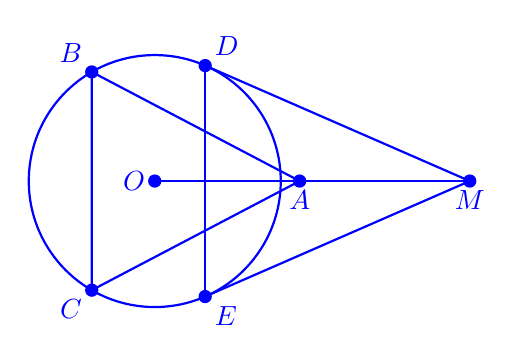
\begin{tikzpicture}[scale=0.8]
    % Định nghĩa tọa độ các điểm
    \coordinate (O) at (0,0);
    \coordinate (A) at (2.3,0);
    \coordinate (B) at (-1,1.732);
    \coordinate (C) at (-1,-1.732);
    \coordinate (M) at (5,0);
    \coordinate (D) at (0.8,1.833);
    \coordinate (E) at (0.8,-1.833);
    
    % Vẽ đường tròn ngoại tiếp (O)
    \draw[blue, thick] (O) circle (2cm);
    
    % Vẽ tam giác ABC
    \draw[blue, thick] (A) -- (B) -- (C) -- cycle;
    
    % Vẽ hai tiếp tuyến từ M
    \draw[blue, thick] (M) -- (D);
    \draw[blue, thick] (M) -- (E);
    
    % Vẽ đoạn thẳng DE
    \draw[blue, thick] (D) -- (E);
    
    % Vẽ đoạn OM
    \draw[blue, thick] (O) -- (M);
    
    % Đánh dấu và ghi nhãn các điểm
    \fill[blue] (O) circle (3pt) node[left] {$O$};
    \fill[blue] (A) circle (3pt) node[below] {$A$};
    \fill[blue] (B) circle (3pt) node[above left] {$B$};
    \fill[blue] (C) circle (3pt) node[below left] {$C$};
    \fill[blue] (M) circle (3pt) node[below] {$M$};
    \fill[blue] (D) circle (3pt) node[above right] {$D$};
    \fill[blue] (E) circle (3pt) node[below right] {$E$};
\end{tikzpicture}
\end{document}